\documentclass[a4paper,11pt]{ltjsarticle}
\usepackage{amsmath, amssymb, amsthm}
\usepackage{tikz-cd}
\usepackage{tikz}
\usetikzlibrary{positioning, arrows.meta, decorations.pathmorphing, calc, shapes.geometric}
\usepackage{hyperref}
\usepackage{tcolorbox}
\tcbuselibrary{skins, breakable}
\usepackage{enumitem}
\usepackage{alltt}

% --- 定理環境 ---
\theoremstyle{definition}
\newtheorem{theorem}{定理}[section]
\newtheorem{lemma}[theorem]{補題}
\newtheorem{definition}[theorem]{定義}
\newtheorem{proposition}[theorem]{命題}
\newtheorem{corollary}[theorem]{系}
\newtheorem{remark}[theorem]{注釈}
\newtheorem{example}[theorem]{例}

% --- tcolorbox スタイル ---
\newtcolorbox{leanbox}[1][]{%
  enhanced, breakable,
  colback=gray!5, colframe=gray!60!black,
  fonttitle=\bfseries\ttfamily,
  title={Lean 4 形式化},
  #1
}

\newtcolorbox{keybox}[1][]{%
  enhanced, unbreakable,
  colback=blue!3, colframe=blue!50!black,
  fonttitle=\bfseries,
  title={核心},
  #1
}

\title{%
  Bourbaki 流「微積分学」の形式化\\[4pt]
  \large --- \texttt{P3\_Calculus} による微分・積分から Fréchet 微分までの俯瞰 ---
}
\author{su}
\date{\today}

\begin{document}

\maketitle

\begin{center}
\small
\textit{AI assistance disclosure:}
Lean ソースコードは Claude (Anthropic) で骨格を生成し、
Codex (OpenAI) で修正した。
\TeX 文書は Gemini 3.1Pro / Antigravity (Google DeepMind) で生成した。
著者による加筆・修正は行っていない。
内容の正確性は保証されず、誤りがあれば著者の責任である。
\end{center}
\begin{abstract}
  Bourbaki 『実一変数関数 (Fonctions d'une variable réelle)』などを背景として、Lean 4 により微積分学の基本定理や中間値の定理をはじめとする解析学の定理群を俯瞰した \texttt{P3\_Calculus.lean} の内容を解説する。
  本稿では、1変数の微分の基礎・平均値の定理・微分積分学の基本定理 (FTC) から出発し、
  さらにノルム空間へ一般化された Fréchet 微分、Taylor 展開、凸解析の初歩へと至る形式化の軌跡を、図式を交えて概観する。
\end{abstract}

\tableofcontents
\newpage

% ===========================================================
\section{導入:微積分学の形式化の全体像}
% ===========================================================

Bourbaki の『実一変数関数』に基づく微積分学の展開は、実数体 $\mathbb{R}$ の位相的・解析的性質の応用として位置づけられる。
本プロジェクトにおける \texttt{P3\_Calculus.lean} は、1変数の微積分から始まり、より一般のノルム空間における微分(Fréchet 微分)へと自然に拡張される構成となっている。

\begin{keybox}
本ファイルで扱われる主要なトピックは以下の通りである。
\begin{itemize}[nosep]
  \item \textbf{微分の演算規則}(線型性、Leibniz 則、連鎖律)
  \item \textbf{平均値の定理}(Rolle の定理、Lagrange の平均値の定理)
  \item \textbf{中間値の定理}(連続関数の性質)
  \item \textbf{微積分学の基本定理 (FTC)}(微分と積分の関係)
  \item \textbf{Fréchet 微分}(ノルム空間への拡張)
  \item \textbf{Taylor の定理と凸解析}(高次微分と関数の大域的性質)
\end{itemize}
\end{keybox}

Mathlib はこれらの定理を極めて一般的な枠組みで提供しているため、本ファイルではそれらを $\mathbb{R}$ 上の関数や一般的なノルム空間の関数に対して適用する形で形式化している。

% ===========================================================
\section{1変数関数の微分と平均値の定理}
% ===========================================================

\subsection{導関数の基礎}

実関数 $f \colon \mathbb{R} \to \mathbb{R}$ の微分可能性は \texttt{DifferentiableAt} によって記述され、その導関数は \texttt{deriv} で与えられる。
\texttt{deriv} は全域で定義された関数を返す設計になっており、微分可能でない点では値が $0$ になるという Mathlib 特有の規約(junk value)を持つ。

\begin{leanbox}
\begin{alltt}
/-- 積の微分法則 (Leibniz rule)。 -/
theorem deriv_mul_at \{f g : \(\mathbb{R} \to \mathbb{R}\)\} \{x : \(\mathbb{R}\)\}
    (hf : DifferentiableAt \(\mathbb{R}\) f x) (hg : DifferentiableAt \(\mathbb{R}\) g x) :
    deriv (f * g) x = deriv f x * g x + f x * deriv g x
\end{alltt}
\end{leanbox}

和・積・合成(連鎖律)といった基本的な演算則は、微分可能性の仮定のもとでそれぞれ
\texttt{deriv\_add}, \texttt{deriv\_mul}, \texttt{deriv\_comp} 等として得られる。

\subsection{Rolle の定理と平均値の定理}

関数の局所的な微分と大域的な変動を結びつける根幹が平均値の定理である。

\begin{theorem}[平均値の定理]
関数 $f$ が閉区間 $[a, b]$ で連続、開区間 $(a, b)$ で微分可能であるとする。このとき、次を満たす $c \in (a, b)$ が存在する。
\[
  f(b) - f(a) = f'(c)(b - a)
\]
\end{theorem}

幾何学的には、割線の傾きと平行な接線を持つ点が区間内に存在することを意味する。

\begin{center}
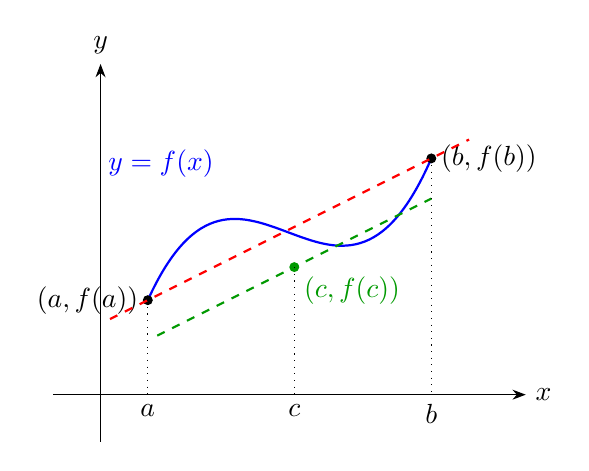
\begin{tikzpicture}[>=Stealth, scale=1.2]
  % Axes
  \draw[->] (-0.5, 0) -- (4.5, 0) node[right] {$x$};
  \draw[->] (0, -0.5) -- (0, 3.5) node[above] {$y$};

  % Curve points
  \coordinate (p0) at (0.5, 1);
  \coordinate (p1) at (1.5, 3.2);
  \coordinate (p2) at (2.5, 0.2);
  \coordinate (p3) at (3.5, 2.5);
  
  % Curve
  \draw[thick, blue] (p0) .. controls (p1) and (p2) .. (p3);
  \node[blue, above left] at (1.3, 2.2) {$y=f(x)$};

  % Points A, B
  \fill (p0) circle (1.5pt) node[left] {$(a, f(a))$};
  \fill (p3) circle (1.5pt) node[right] {$(b, f(b))$};

  % Secant line
  \draw[red, thick, dashed] (0.1, 0.8) -- (3.9, 2.7);
  
  % Tangent line approximation
  \coordinate (c) at (2.05, 1.35); 
  \coordinate (t1) at (0.6, 0.625);
  \coordinate (t2) at (3.5, 2.075);
  \draw[green!60!black, thick, dashed] (t1) -- (t2);
  \fill[green!60!black] (c) circle (1.5pt) node[below right] {$(c, f(c))$};

  % Drop lines
  \draw[dotted] (0.5, 1) -- (0.5, 0) node[below] {$a$};
  \draw[dotted] (3.5, 2.5) -- (3.5, 0) node[below] {$b$};
  \draw[dotted] (2.05, 1.35) -- (2.05, 0) node[below] {$c$};
\end{tikzpicture}
\end{center}

\begin{leanbox}
\begin{alltt}
theorem mean_value_theorem \{f : \(\mathbb{R} \to \mathbb{R}\)\} \{a b : \(\mathbb{R}\)\} (hab : a < b)
    (hfc : ContinuousOn f (Icc a b))
    (hfd : \(\forall\) x \(\in\) Ioo a b, DifferentiableAt \(\mathbb{R}\) f x) :
    \(\exists\) c \(\in\) Ioo a b, f b - f a = deriv f c * (b - a)
\end{alltt}
\end{leanbox}

Lean 4 実装では、この定理から「導関数が常に非負ならば関数は単調非減少である」という事実 (\texttt{monotone\_of\_deriv\_nonneg}) が導出される。

% ===========================================================
\section{中間値の定理と微積分学の基本定理}
% ===========================================================

\subsection{中間値の定理 (Intermediate Value Theorem)}

連続関数の性質として、連結な領域の像が再び連結になるという事実から、中間値の定理が得られる。
\texttt{intermediate\_value\_Icc} によって示され、その系として Bolzano の零点定理が導かれる。

\begin{leanbox}
\begin{alltt}
/-- 零点定理 (Bolzano): f(a) < 0 < f(b) ならば零点が存在。 -/
theorem bolzano \{f : \(\mathbb{R} \to \mathbb{R}\)\} \{a b : \(\mathbb{R}\)\} (hab : a \(\le\) b)
    (hf : ContinuousOn f (Icc a b))
    (ha : f a < 0) (hb : 0 < f b) :
    \(\exists\) c \(\in\) Icc a b, f c = 0
\end{alltt}
\end{leanbox}

\subsection{微積分学の基本定理 (FTC)}

微分と積分の互換性を保証する微積分学の基本定理 (Fundamental Theorem of Calculus) は、解析学における最も重要な成果の一つである。
本形式化では、以下の2つの部分に分けて示される。

\begin{center}
\begin{tikzcd}[column sep=huge, row sep=large]
  \left\{ \text{連続関数 } f \right\}
  \arrow[r, bend left=15, "\text{積分 } F(x) = \int_a^x f(t) \,dt"]
  & \left\{ \text{可微分関数 } F \right\}
  \arrow[l, bend left=15, "\text{微分 } F'(x)"]
\end{tikzcd}
\end{center}

\begin{itemize}
  \item \textbf{第1基本定理 (\texttt{ftc\_part1})}:連続関数を積分して得られる関数は微分可能であり、その導関数は元の関数に一致する。
  \item \textbf{第2基本定理 (\texttt{ftc\_part2})}:導関数が $f$ であるような原始関数 $F$ を用いて、定積分を $F(b) - F(a)$ として計算できる (Newton-Leibniz 公式)。
\end{itemize}

\begin{leanbox}
\begin{alltt}
theorem ftc_part2 \{a b : \(\mathbb{R}\)\} \{F : \(\mathbb{R} \to \mathbb{R}\)\}
    (hF : \(\forall\) x \(\in\) uIcc a b, HasDerivAt F (f x) x)
    (hf : IntervalIntegrable f MeasureTheory.volume a b) :
    \(\int\) x in a..b, f x = F b - F a
\end{alltt}
\end{leanbox}

% ===========================================================
\section{多変数・ノルム空間への一般化:Fréchet 微分}
% ===========================================================

Bourbaki の多様体論への準備として、微分概念はノルム空間 $E, F$ の間の写像へと拡張される。
関数 $f \colon E \to F$ が $x \in E$ で \textbf{Fréchet 微分可能} であるとは、ある有界線型作用素 $L \in \mathcal{L}(E, F)$ が存在して、
\[
  f(x + h) - f(x) = L(h) + o(\|h\|) \quad (h \to 0)
\]
を満たすことである。この $L$ を $f$ の $x$ における Fréchet 微分といい、\texttt{fderiv} で表す。

\begin{theorem}[連鎖律 (Chain Rule)]
ノルム空間間の写像の合成 $f \circ g$ の Fréchet 微分は、各写像の Fréchet 微分の合成(線型作用素の合成)となる。
\end{theorem}

\begin{center}
\begin{tikzcd}[column sep=large, row sep=large]
  E \arrow[r, "g"] \arrow[rr, bend left=25, "f \circ g"]
  & F \arrow[r, "f"]
  & G \\
  E \arrow[r, "d_x g"'] \arrow[rr, bend right=25, "d_x(f \circ g)"']
  & F \arrow[r, "d_{g(x)} f"']
  & G
\end{tikzcd}
\end{center}

\begin{leanbox}
\begin{alltt}
theorem fderiv_comp_at \{f : F \(\to\) G\} \{g : E \(\to\) F\} \{x : E\}
    (hf : DifferentiableAt \(\mathbb{R}\) f (g x)) (hg : DifferentiableAt \(\mathbb{R}\) g x) :
    fderiv \(\mathbb{R}\) (f \(\circ\) g) x = (fderiv \(\mathbb{R}\) f (g x)).comp (fderiv \(\mathbb{R}\) g x)
\end{alltt}
\end{leanbox}

% ===========================================================
\section{テイラーの定理から凸解析まで}
% ===========================================================

ファイルの終盤では、さらに高度な解析の話題が提示されている。

\subsection{Taylor展開と解析関数}

Taylor の定理は、関数を多項式によって近似する強力なツールである。指数関数 $\exp(x)$ のマクローリン展開に関する収束定理など、具体的な解析関数の性質も Mathlib を使って自然に表現できる。

\subsection{陰関数定理と凸解析}

また、微分を用いた幾何学的性質の解析として、以下への展望が示されている。
\begin{itemize}
  \item \textbf{逆関数定理・陰関数定理}:局所的な同相性や、方程式の解の曲面・多様体としての振る舞いを決定する。
  \item \textbf{凸解析 (Convex Analysis)}:関数 $f$ の凸性と導関数 $f'$ の単調性が結びつき、Jensen の不等式などに至る。
\end{itemize}

これらの抽象的な理論体系は、関数解析や多様体論への堅固な礎(正に母構造の応用)を提供するものである。

\end{document}
